%% LyX 2.0.5.1 created this file.  For more info, see http://www.lyx.org/.
%% Do not edit unless you really know what you are doing.
\documentclass[usenatbib]{article}
\usepackage[latin9]{inputenc}
\usepackage[a4paper]{geometry}
\geometry{verbose}
\usepackage{color}
\usepackage{float}
\usepackage{graphicx}

\makeatletter

%%%%%%%%%%%%%%%%%%%%%%%%%%%%%% LyX specific LaTeX commands.
%% Because html converters don't know tabularnewline
\providecommand{\tabularnewline}{\\}
%% A simple dot to overcome graphicx limitations
\newcommand{\lyxdot}{.}


%%%%%%%%%%%%%%%%%%%%%%%%%%%%%% Textclass specific LaTeX commands.
\usepackage{jcappub}

%%%%%%%%%%%%%%%%%%%%%%%%%%%%%% User specified LaTeX commands.






%%%%%%%%%%%%%%%%%%%%%%%%%%%%%% LyX specific LaTeX commands.
%% A simple dot to overcome graphicx limitations
%Make my life significantly easier
\usepackage{lineno}\global\long\def\bd{{\bm{\delta}}}
\usepackage{astrobib_mnras2e}
\linenumbers

\makeatother

\begin{document}

\title{Generating Mock Catalogs for the Baryon Oscillation Spectroscopic
Survey: An Approximate N-Body approach}


\author{Tomomi Sunayama\textsuperscript{a}, Nikhil Padmanabhan\textsuperscript{a},
Katrin Heitmann\textsuperscript{b}, Salman Habib\textsuperscript{b},
Steve Rangel\textsuperscript{b,c}}


\abstract{Precision large scale structure measurements require large numbers
of mock catalogs of high fidelity to accurately assess the levels
of systematic effects. We introduce and test an approximate scheme
for generating mock catalogs rapidly. Our aim here is to reproduce
the large scale structure and the gross properties of dark matter
halos with high accuracy while sacrificing the details of the internal
structures of halos for speed. Our N-body code splits the evolution
into global time steps for the long range force interleaved with a
number of sub-cycles for the short range forces. By adjusting both
of these, we demonstrate recover the large scale probes we consider,
including individual halo masses to better than 2\% and the power
spectrum to $k=1h^{-1}{\rm Mpc}$ to better than 1\%, while requireing
a factor of 4 less CPU time. We also test the redshift spacing of
outputs required to generate light cone outputs. We find that $\Delta z=0.05$
outputs allow us to interpolate particle positions and velocities
with sufficient accuracy to reproduce the real and redshift space
power spectra to better than 1\% (out to $k=1h^{-1}{\rm Mpc}$). Even
with redshift spacing as large as $\Delta z=0.25$, these errors only
degrade on less than 2\% in both real and redshift spaces. As a demonstration
of these ideas, we generate a suit of simulations matched to the Baryon
Oscillation Spectroscopic sample.}


\affiliation{\textsuperscript{a}Yale University, New Haven, CT}


\affiliation{\textsuperscript{b }Argonne National Laboratory, Lemont, IL}


\affiliation{\textsuperscript{c }Northwestern University, Evanston, IL}

\maketitle

\section{Introduction}

Recently, the necessity and the demand for the large number of large
N-body simulations have been increased in astronomy due to the precision
required for measurements to understand cosmic acceleration, like
the Baryon Oscillation Spectroscopic Survey (BOSS) and the proposed
Mid Scale-Dark Energy Spectroscopic Instrument (MS-DESI). As the area
covered by those current and future spectroscopic galaxy surveys get
larger, galaxy mocks necessary to the cosmological analysis also have
to be generated from N-body simulations with the corresponding large
volume, which is computationally expensive. Many studies have been
done recently on the implementation of large N-body simulations \cite{2002ApJ...564....8M,2002MNRAS.331..587M,2008MNRAS.391..435F,2013AN....334..691R,2013arXiv1312.2013C,2013JCAP...06..036T,2014MNRAS.437.2594W,2013MNRAS.433.2389M,2001A&A...367...18H,2009ApJ...701..945S,2014MNRAS.439L..21K,2014arXiv1409.1124C}.
Besides the large volume required for the N-body simulations, we need
many realizations to achieve the precision required for those measurements.

One of the simplest adjustments to an N-body simulation is to adjust
the length of each individual time step. This is the approach taken
in \cite{2014MNRAS.437.2594W,2013JCAP...06..036T}; indeed, the 2LPT
mock simulations of \cite{2013MNRAS.428.1036M,2014arXiv1401.4171M}
are an extreme version of this. These works have focused on relatively
small numbers of time steps, accurately capturing the large scale
density field, but losing information on small scales. While such
approaches are invaluable for generating the large numbers of simulations
required to build sample covariance matrices, it is harder to quantify
the impact of the loss of accuracy on systematic tests. Our N-body
simulations are consist of two components: a long time step for solving
the PM force and a set of short range sub-cycle steps for a direct
particle-particle interaction. The idea behind is reducing the number
of both time steps as much as we can preserve enough mass resolution
to correctly describe the large scale distribution of galaxies. Our
first goal in this paper is to work at a different end of the spectrum
: we aim to accurately reproduce the details of the halo density field
on large scales, sacrificing the small scale structure with large
time steps. Our second goal, is to build a suite of simulations and
related mock catalogs suitable for the Baryon Oscillation Spectroscopic
Survey galaxy samples. These both serve as a demonstration of our
approach, but will be useful for evaluating systematic errors in these
surveys.

In the following, we first briefly describe the mechanism of our approximated
N-body simulations. In Section 3, we test and compare our method to
the full N-body simulation and explain how we calibrate our samples.
In Section 4 and 5, we build a light cone output and populate halos
in our samples with galaxies and compute correlation functions based
on BOSS Data Release 11, and compare it with the observed correlation
function.

All simulations and calculations in this paper assume a $\Lambda$CDM
cosmology with $\Omega_{m}=0.25$, $\Omega_{\Lambda}=0.75$, $\Omega_{b}h^{2}=0.0224$,
$n_{s}=0.97$, $\sigma_{8}=0.8$ and $h=0.72$.


\section{HACC}

All simulations in this paper were carried out using the HACC (Hardware/Hybrid
Accelerated Cosmology Code) framework. HACC provides an advanced,
architecture-agile, extreme-scale N-body capability targeted to cosmological
simulations. It is descended from an approach originally developed
for the heterogeneous architecture of Roadrunner~\cite{mc3,pope10},
the first computer to break the petaflop performance barrier.

The HACC architecture is designed with great flexibility in mind (combining
MPI with a variety of more local programming models, e.g., OpenCL,
OpenMP) and is easily adaptable to different platforms. Currently,
it is implemented on Cell-accelerated hardware, conventional and GPU-enhanced
clusters (via OpenCL), on the IBM Blue Gene architecture (using OpenMP),
and is running on prototype Intel MIC/Xeon Phi hardware. HACC is the
first, and currently the only large-scale cosmology code suite world-wide,
that can run at full scale on all available supercomputer architectures,
at very high performance levels. HACC has demonstrated scaling on
the entire IBM BG/Q Sequoia system up to 1,572,864 cores with an equal
number of MPI ranks, attaining 13.94 PFlops at 69.2\% of peak and
90\% parallel efficiency (for details, see Ref.~\cite{habib12}).
Examples of science results obtained using HACC include 64-billion
particle runs for baryon acoustic oscillations predictions for the
BOSS Lyman-$\alpha$ forest~\cite{boss_bao} and high-statistics
predictions for the halo profiles of massive clusters~\cite{conc_hacc}.

HACC uses a hybrid parallel algorithmic structure, splitting the force
calculation into a specially designed grid-based long/medium range
spectral particle-mesh (PM) component that is common to all architectures,
and an architecture-specific short-range solver. Modular code design
combined with particle caching allows the short-range solvers to be
`hot-swappable' on-node; they are blind to the parallel implementation
of the long-range solver. The short-range solvers can use direct particle-particle
interactions, i.e., a P$^{3}$M algorithm~\cite{hockney}, as on
(Cell or GPU) accelerated systems, or use tree methods on conventional
or many-core architectures. (This was the case for the simulations
reported here.) In all cases, the time-stepping scheme is based on
a symplectic method with (adaptive) sub-cycling of the short-range
force. The availability of multiple algorithms within the HACC framework
allows us to carry out careful error analyses, for example, the P$^{3}$M
and the TreePM versions agree to within $0.1\%$ for the nonlinear
power spectrum test in the code comparison suite of Ref.~\cite{heitmann05}.

An important feature of the work proposed here is the ability to carry
out error-controlled approximate simulations at high throughput. In
order to understand how we implement this, some details of the HACC
time-stepping algorithm are now provided. Evolution is viewed as a
symplectic map on phase space: $\zeta(t)=\exp(-t{\bf {H}})\zeta(0)$
where, $\zeta$ is a phase-space vector $({\bf x},{\bf v})$, $H$
is the (self-consistent) Hamiltonian, and the operator, ${\bf {H}}=[H,~]_{P}$,
denotes the action of taking the Poisson bracket with the Hamiltonian.
Suppose that the Hamiltonian can be written as the sum of two parts;
then by using the Campbell-Baker-Hausdorff (CBH) series we can build
an integrator for the time evolution; repeated application of the
CBH formula yields 
\[
\exp(-t({\bf {H}}_{1}+{\bf {H}}_{2}))=\exp(-(t/2){\bf {H}}_{1})\exp(-t{\bf {H}}_{2})\exp(-(t/2){\bf {H}}_{1})+O(t^{3}),
\]
a second order symplectic integrator. In the basic PM application,
the Hamiltonian $H_{1}$ is the free particle (kinetic) piece while
$H_{2}$ is the one-particle effective potential; corresponding respectively
to the `stream' and `kick' maps $M_{1}=\exp(-t{\bf {H}}_{1})$ and
$M_{2}=\exp(-t{\bf {H}}_{2})$. In the stream map, the particle position
is drifted using its known velocity, which remains unchanged; in the
kick map, the velocity is updated using the force evaluation, while
the position remains unchanged. This symmetric `split-operator' step
is termed SKS (stream-kick-stream). A KSK scheme constitutes an alternative
second-order symplectic integrator.

In the presence of both short and long-range forces, we split the
Hamiltonian into two parts, $H_{1}=H_{sr}+H_{lr}$ where $H_{sr}$
contains the kinetic and particle-particle force interaction (with
an associated map $M_{sr}$), whereas, $H_{2}=H_{lr}$ is just the
long range force, corresponding to the map $M_{lr}$. Since the long
range force varies relatively slowly, we construct a single time-step
map by sub-cycling $M_{sr}$: $M_{full}(t)=M_{lr}(t/2)(M_{sr}(t/n_{c}))^{n_{c}}M_{lr}(t/2)$,
the total map being a usual second-order symplectic integrator. This
corresponds to a KSK step, where the S is not an exact stream step,
but has enough $M_{sr}$ steps composed together to obtain the required
accuracy. (We take care that the time-dependence in the self-consistent
potential is treated correctly.) As discussed later below, we will
use the flexibility in the sub-cycling as a way of reducing the number
of time steps such that the loss of accuracy only affects the resolution
at very small scales, which, as discussed previously, are not of interest
in the current set of simulations.


\section{Convergence Test: Selection of the minimal time steps}

In this section, we examine how reducing the number of time steps
affects halo properties (i.e., halo mass, position, and velocity),
as well as observables such as halo mass functions and halo bias.
In order to quantitatively evaluate different time-stepping options,
we run a set of convergence tests with down-scaled simulation boxes,
using simulation volumes of size $(256h^{-1}{\rm Mpc})^{3}$ and $256^{3}$
particles. These runs have the same particle mass as the main $(4000h^{-1}{\rm Mpc})^{3}$
volume simulations.

Time-stepping convergence was studied using the following time step
options: 450/5, 300/3, 300/2, 150/3, and 150/2, where the first number
indicates the number of long time steps and the second number the
number of short sub-time steps for each long time step. To evaluate
the different time-stepping options, we first compare the properties
(masses, positions, and velocities) of individual halos by matching
halos in one simulation run to halos in another, using identical initial
conditions, and with adaptive time-stepping switched off. Following
this, we compare statistical descriptions such as halo mass functions
and density power spectra. We found that, for the purpose of the work
presented in this paper, differences in halo properties do not significantly
affect the statistical observables. Based on a number of convergence
tests, the 300/2 time-stepping option was found sufficient to resolve
the positions and masses of halos reliably.


\subsection{Matching }

In order to compare compare detailed halo properties we need to match
individual halos across different runs. We first discuss the algorithm
used for identifying the corresponding halos in the two cases and
then compare halo mass, position, and velocity for the matched halos.
From this quantitative comparison, we find that the simulations with
300 global time steps have significantly less scatter in the measured
quantities, compared to the baseline determined by the 450/5 simulation,
than do the samples with 150 global steps. In addition, we find that
the differences between the different sub-cycling choices are almost
negligible.


\subsubsection{Algorithm}

All the simulations start with the same particle initial conditions,
therefore we match halos in different runs by matching their particle
content, using individual particle identification. Given a halo in
simulation A, we consider halos in simulation B that between them
hold all the particles belonging to the halo in simulation A. Given
this list of possible matches, we choose the run B halo with the largest
number of common particles with the reference halo in run A. To avoid
spurious matches, we also require that the fraction of common particles
(relative to simulation A) exceeds a given threshold. To illustrate
how this matching algorithm works, we use the samples from the 300/2
simulation and the 450/5 simulation, and adopt a threshold of 50\%
as our default choice. (Figure \ref{fig:mass-content} demonstrates
that the unmatched fraction increases with increasing threshold and
decreasing halo mass.)

The matching algorithm described above is unidirectional, hence multiple
halos in run A may have particles resident in a single halo in run
B; in our simulations, this happens at the 1-2\% level, adopting a
particle matching threshold of 50\%. We refer to these cases as `multiply-booked'
halos. Figure~\ref{fig:mass-scatter1} compares halo masses matching
the 450/5 simulation to the 300/2 simulation for the case of multiply-booked
halos as well as the rest. The top left panel shows the mass scatter
for all the matched halos between the two simulations, while the top
right panel shows the mass scatter only for the non multiply-booked
halos. The bottom panels show the mass scatter for the case of multiply-booked
halos only. The bottom left panel shows the mass scatter for individual
multiply-booked halos, while the bottom right panel plots the summed
halo mass for the corresponding halos. The overall behavior represented
in Figure~\ref{fig:mass-scatter1} is straightforward to interpret.

\begin{figure}[h]
\includegraphics[width=0.465\columnwidth]{\lyxdot \lyxdot /Plots/testDB_mass_300_2_z0\lyxdot 15}
\includegraphics[width=0.535\columnwidth]{\lyxdot \lyxdot /Plots/testDB_nonDB_300_2_z0\lyxdot 15}

\includegraphics[width=0.465\textwidth]{\lyxdot \lyxdot /Plots/testDB_DB_numPartCut_300_2_z0\lyxdot 15}
\includegraphics[width=0.535\columnwidth]{\lyxdot \lyxdot /Plots/testDB_sum_mass_f0\lyxdot 5_300_2_z0\lyxdot 15}

\caption{\label{fig:mass-scatter1}Distribution of halo masses comparing matched
halos in the 450/5 simulation (x-axis) to the 300/2 simulation (y-axis)
at $z=0.15$. Panels correspond to halos with different matching criteria
imposed: all the matched halos (top left), the vast majority of matched
halos having one-to-one correspondence (top right), matched halos
not having one-to-one correspondence called ``multiply-booked''
halos (bottom left), and the ``multiply-booked'' halos whose corresponding
halo masses are added (bottom right). The results shown in these panels
imply that the low-mass scatter between the 450/5 simulation and the
300/2 simulation shown in the top left panel arises when``multiply-booked''
halos in the 450/5 simulation are merged into one halo in the 300/2
simulation due to an effectively worse resolution in this case.}
\end{figure}


As the top left panel shows, there are low-mass halos in the 450/5
simulation corresponding to high-mass halos in the 300/2 simulation.
The same trend is observed for the case of multiply-booked halos (bottom
left panel), but not for the non multiply-booked halos (top right).
Furthermore, the disagreement for halo masses between the two simulations
are resolved by adding the corresponding halo masses. This implies
that there are multiple halos in the 450/5 simulation which are merged
into one halo in the 300/2 simulation. The smaller number of time
steps in the 300/2 simulations reduces substructure and as well as
the compactness of the halos in the 450/5 simulation. Thus, for a
small fraction of halos in the 450/5 simulation, individual halos
can be merged into a single halo in the 300/2 simulation.

Figure \ref{fig:mass-content} shows the number densities of the unmatched
halos in the 450/5 simulation when compared to the 300/2 simulation
at $z=0.15$. There are three reasons that halos can turn up as unmatched.
In the first case, particles forming a halo in simulation A may not
form a component of a halo in simulation B (no common particles).
Second, if the fraction of common particles over the total number
of particles in each halo is less than the threshold of 50\%, these
halos will be eliminated from the matching set. Finally, for the case
of multiply-booked halos, we remove all but the one with the largest
number of common particles. In Figure \ref{fig:mass-content}, we
show each type of unmatched number density as a function of halo mass.
The first case occurs only for low halo masses, where low effective
resolution in a simulation can lead to halo drop out (halos are too
'fuzzy' to meet the FOF overdensity criterion), and falls off steeply
with rising halo mass. Most of the unmatched halos arise due to their
not passing the threshold criterion. The loss of matching due to multiple-booking
follows the trend of the below-threshold case, but at a reduced level.
We have checked that the trends discussed here are not affected by
redshift.

\begin{figure}[H]
\includegraphics[width=0.5\columnwidth]{\lyxdot \lyxdot /Plots/unmatchHalo2_content_300_2_z0\lyxdot 15}

\caption{\label{fig:mass-content} Itemization of unmatched halos (from the
450/5 and 300/2 simulations at $z=0.15$) shown as cumulative number
densities of the unmatched halos arising from each procedure in the
matching algorithm. The solid blue line is the total number density
of the unmatched halos. The dashed green line shows halos with no
counterpart -- none of the particles were identified as belonging
to a halo in the comparison simulation; this is significant only at
low halo mass. The dashed red line shows halos eliminated because
of not meeting the matching threshold (i.e., the halos do not have
enough of a fraction of the same particles). The dashed cyan line
is for the halos eliminated because multiple halos correspond to one
halo. }
\end{figure}



\subsubsection{Halo Properties}

We now compare halo properties (i.e., halo mass, position, and velocity)
for the 300/2 halos that were successfully matched to those in the
450/5 simulation. We are interested in correctly describing the large-scale
distribution of galaxies; in the current context, this requires that
dark matter halo locations and masses be estimated sufficiently accurately.
Therefore, it is essential to systematically investigate the effect
of reducing the number of time steps on halo properties.

The comparison of halo mass for different time-stepping schemes to
the 450/5 simulation at $z=0.15$ is shown in Figure \ref{fig:HaloProperty_mass}.
We take all the matched halos whose masses are between $10^{12.5}{\rm M_{\odot}}$
to $10^{13.0}{\rm M_{\odot}}$, $10^{13.0}{\rm M_{\odot}}$ to $10^{13.5}{\rm M_{\odot}}$,
and $10^{13.5}{\rm M_{\odot}}$ to $10^{14.0}{\rm M_{\odot}}$, and
compute their means and standard deviations for ${\rm log_{10}(M/M_{450/5})}$,
where $M_{450/5}$ is a halo mass for the 450/5 simulation and $M$
corresponds to a halo in the samples generated with different time-stepping
schemes. Figure \ref{fig:HaloProperty_mass} shows that halos generated
from the simulations with small number of time steps have systematically
lower FOF masses than those in the 450/5 simulation. (The same linking
length ($b=0.168$) is used in the FOF algorithm to define halos for
all the simulations.) As stated earlier, reducing the number of time
steps produces halos with less substructure and a more diffuse distribution
of mass, thus in a direct one-on-one halo comparison, one expects
the FOF mass to be highest in the 450/5 simulation, as borne out in
the data. 

Figure~\ref{fig:HaloProperty_step} shows the differences in positions
(left panel) and velocities (right panel) along x-axis for the matched
halos at $z=0.15$. The simulations with a smaller number of global
time steps (150) display significantly more scatter; they also show
a small bias in the speed. With 300 global time steps, the results
are significantly improved; the velocity bias is almost entirely removed
and the scatter is significantly reduced. The standard deviation in
the differences in halo distances is matched in these cases to better
than $200h^{-1}{\rm kpc}$\textcolor{black}{. The dashed lines represent
the result from the simulations, while the solid lines are the Gaussian
fits, where the values for amplitude, expected value and variance
are shown in Table \ref{tab:amplitude}. Figure \ref{fig:HaloProperty_step}
shows that the distribution of the differences in positions and velocities
are almost Gaussian.} As is clear from Figure \ref{fig:HaloProperty_step},
the difference between 3 and 2 sub-cycles is negligible on halo properties.
Note that we observe the same trend in halo properties discussed here
at different redshifts and along different axes. 

\textcolor{black}{As shown in Figure \ref{fig:mass-content}, the
fraction of unmatched halos in the 300/2 simulation to the 450/5 simulation
is less than 5\% on most of halo mass ranges, which implies that the
300/2 simulation has almost the same number of halos as in the 450/5
simulation. Furthermore, Figure \ref{fig:mass-scatter1} shows that
the halo masses in the 450/5 and 300/2 simulations have linear relation
with the slope being one. So, most of halos in the 300/2 simulation
have the same mass as the ones in the 450/5 simulation. Since the
number of sub-cycles do not affect to halo positions and velocities
as shown in Figure \ref{fig:HaloProperty_step}, the 300/2 time step
is our choice to save the simulation time while keeping the halo properties
almost identical to the 450/5 simulation.}

\textcolor{black}{}
\begin{figure}[h]
\textcolor{black}{\includegraphics[width=0.5\columnwidth]{\lyxdot \lyxdot /Plots/massSlice_z0\lyxdot 15}}

\textcolor{black}{\caption{\label{fig:HaloProperty_mass}Comparison of halo mass for matched
halos between the 450/5 simulation and other time-stepping schemes
at $z=0.15$. We take all the matched halos whose masses are between
$10^{12.5}{\rm M_{\odot}}$ to $10^{13.0}{\rm M_{\odot}}$, $10^{13.0}{\rm M_{\odot}}$
to $10^{13.5}{\rm M_{\odot}}$, and $10^{13.5}{\rm M_{\odot}}$ to
$10^{14.0}{\rm M_{\odot}}$, and compute the mean and the standard
deviation for ${\rm log_{10}(M/M_{450/5})}$ where $M_{450/5}$ is
a halo mass for the 450/5 simulation and $M$ is for the simulations
with different number of time steps corresponding to different colors
in the plot. The x-positions of the points have been displaced to
avoid overlapping the error bars. This plot shows that halo masses
become systematically smaller for the case of smaller numbers of time
steps than those in the 450/5 simulation. }
}
\end{figure}


\begin{figure}[h]
\includegraphics[width=0.5\columnwidth]{\lyxdot \lyxdot /Plots/histogram_x_z0\lyxdot 15}\includegraphics[width=0.5\columnwidth]{\lyxdot \lyxdot /Plots/histogram_vx_z0\lyxdot 15}

\caption{\label{fig:HaloProperty_step}A comparison of the positions {[}left{]}
and velocities {[}right{]} of halos matched across simulations with
different time steps. As always, the reference simulation is 450/5
while the colors correspond to 300/3 (blue), 300/2 (green), 150/3
(red), and 150/2 (cyan). From left to right, we compared halo position
and velocity respectively.\textcolor{blue}{{} }\textcolor{black}{The
agreement with 300 time steps is very good, with a negligible difference
from the number of sub-cycles. }}
\end{figure}


\begin{table}
\begin{tabular}{|c|c|c|c|}
\hline 
 & $A$ & $\mu$ & $\sigma$\tabularnewline
\hline 
\hline 
300/3 & 3377.2 & 0.0 & 0.0715\tabularnewline
\hline 
300/2 & 2937.2 & 0.0 & 0.0781\tabularnewline
\hline 
150/3 & 1280.9 & 0.0 & 0.1709\tabularnewline
\hline 
150/2 & 1077.4 & 0.0 & 0.1783\tabularnewline
\hline 
\end{tabular} %
\begin{tabular}{|c|c|c|c|}
\hline 
 & $A$ & $\mu$ & $\sigma$\tabularnewline
\hline 
\hline 
300/3 & 3461.5 & -3.138 & 11.527\tabularnewline
\hline 
300/2 & 1975.8 & -3.105 & 12.780\tabularnewline
\hline 
150/3 & 1975.0 & -15.660 & 17.955\tabularnewline
\hline 
150/2 & 1667.7 & -15.821 & 18.592\tabularnewline
\hline 
\end{tabular}

\caption{\label{tab:amplitude}Values for amplitude $A$, expected value $\mu$,
variance $\sigma$ in Gaussian fits shown in Figure \ref{fig:HaloProperty_step}
for the positions {[}right{]} and velocities {[}left{]} across simulations
with different time steps. Note that we specifically fit the distribution
of position differences with the expected value 0.}
\end{table}



\subsection{Mass Adjustment}

In the previous subsection, Figure \ref{fig:HaloProperty_mass} shows
that halos generated by the de-tuned simulations have systematically
lower masses than the halos in the 450/5 simulation. This suggests
the necessity of adjusting halo masses for those cases to the halo
masses in the 450/5 simulation. In the following, we describe how
we do a mass adjustment and show the resulting observables including
mass functions and power spectra.


\subsubsection{Method}

To calibrate halo masses for the simulations with the reduced number
of time steps, we first take all the matched halos between the 450/5
simulation and the de-tuned simulations and compute means for each
mass bin. We consider only the matched halos is because the aim of
the mass adjustment is to correct systematic mass differences for
the halos that are theoretically identical in the different runs.
After computing the means for each mass bin, we fit them to a functional
form that brings the reassigned halo mass, $M_{re}$, close to the
average halo mass for the 450/5 simulation. For our simulations, we
find that the following simple form suffices for this task:

\begin{equation}
M_{re}=M(1.0+\alpha(M/10^{12.0}[{\rm M_{\odot}])^{\beta},}\label{eq:mass_adjust}
\end{equation}
where $M_{re}$ is the reassigned halo mass, $M$ is the original
halo mass, and $\alpha$ and $\beta$ are free parameters. The $\alpha$
and $\beta$ values for the simulations with different numbers of
time steps are listed in Table \ref{tab:free_param1} (at $z=0.15$).

\begin{table}
\begin{tabular}{|c|c|c|}
\hline 
 & $\alpha$  & $\beta$\tabularnewline
\hline 
\hline 
300/3  & 0.005  & 0.175\tabularnewline
\hline 
300/2  & 0.07  & -0.47\tabularnewline
\hline 
150/3  & 0.101  & -0.162\tabularnewline
\hline 
150/2  & 0.315  & -0.411\tabularnewline
\hline 
\end{tabular}

\caption{\label{tab:free_param1}The mass reassignment parameters $\alpha$
and $\beta$ of Eq.~\ref{eq:mass_adjust} for simulations run with
different numbers of time steps (the results are shown at $z=0.15$).}
\end{table}


The best-fit parameters $\alpha$ and $\beta$ are functions of redshift.
For the case of the 300/2 simulation, we find best fit parameters
shown below:

\begin{equation}
\alpha(z)=0.123z+0.052,
\end{equation}
and 
\begin{equation}
\beta(z)=-0.154z-0.447.
\end{equation}



\subsubsection{Observables}

Now, we show mass functions and power spectra for the different simulations
after applying the mass adjustment.

We first compute mass functions from outputs of different time-stepping
schemes, as shown in Figure \ref{fig:massFn_step}, where we compare
simulations with reduced number of time steps to the 450/5 simulation
at $z=0.15$. In Figure \ref{fig:massFn_step}, we show the ratio
$n(>M)/n_{450/5}(>M)$, where $n_{450/5}(>M)$ is a cumulative mass
function for the 450/5 simulation and $n(>M)$ is a cumulative mass
function for different time steps shown in different colors. We compare
the results before and after mass adjustment (left and right panels
respectively). While the mass functions from the 250/3 and 150/2 simulations
are suppressed more than 10\% on all mass ranges before mass adjustment,
they are significantly improved after mass adjustment, especially
on halo masses greater than $10^{13.0}{\rm M_{\odot}}$. For the simulations
with the 300 global time steps, mass adjustment is especially effective
on small halo masses.

\begin{figure}[H]
\includegraphics[width=0.5\columnwidth]{\lyxdot \lyxdot /Plots/haloRatioNum256_z0\lyxdot 15}
\includegraphics[width=0.5\columnwidth]{\lyxdot \lyxdot /Plots/haloRatioNum256_tweak_z0\lyxdot 15}

\caption{\label{fig:massFn_step} Comparison of cumulative mass functions in
different simulations taking the 450/5 simulation as a reference.
Lines, from top to bottom, correspond to the simulation with different
time steps, 300/3 (blue), 300/2 (green), 150/3 (red), and 150/2 (cyan)
respectively. The left panel shows the cumulative mass functions before
adjusting masses (as described in the text), while the right panel
is after. These plots demonstrate that a simple mass recalibration
allows one to successfully recover the mass functions, even in the
extreme case of the 150/2 simulation, which differed by more than
10\% (on all mass scales). }
\end{figure}


The next measure of interest is halo-matter cross power spectra between
halo and matter density fields, as shown in Figure \ref{fig:crossMater_step}.
Figure \ref{fig:crossMater_step} shows the ratio $P_{hm}/P_{hm,450/5}$
at $z=0.15$, where $P_{hm,450/5}$ is the cross power spectrum for
the 450/5 simulation and $P_{hm}$ is the cross power spectrum for
other time steps corresponding to different colors, as labeled in
Figure \ref{fig:crossMater_step}. We use the real-space halo density
field for the left panel and the redshift-space halo densities for
the right panel in Figure \ref{fig:crossMater_step}. For the dark
matter density field, we use the output of the 450/5 simulation for
all the halo samples. Note that the dark matter density fields are
in real-space for both cases. In this way, the ratio $P_{hm}/P_{hm,450/5}$
in real-space i\textcolor{black}{s equivalent to the ratio of halo
bias between the 450/5 simulation and the simulations with other time-steps.
To select halos, we apply the soft-mass cut method using the probability
given by }

\textcolor{black}{
\begin{equation}
<N_{halo}(M)>=\frac{1}{2}{\rm erfc}(\frac{{\rm log(M_{cut}/}M)}{\sqrt{2}\sigma}),
\end{equation}
where we set ${\rm M_{cut}=10^{13.0}[{\rm M_{\odot}]}}$ and $\sigma=0.5$.
This probability has a similar form to the halo occupation distribution
(hereafter, HOD) technique so that the probability gradually becomes
one as increasing halo mass. We use this method to avoid noise from
halos scattering across sharp boundaries on halo mass.} Note that
the errors calculated here are not due to sample variance, because
we generate 10 samples from one full sample by using the soft-mass
cut method. We see that, as we decrease the number of time steps,
the ratio of the cross power spectra increases, especially in redshift-space,
we observe large deviations from one on small scales for the 150/2
and 150/3 simulations. This is due to the overall smaller halo velocities
for those simulations, which is shown in Figure \ref{fig:HaloProperty_step}.
For the simulations with the 300 global time steps, overall agreements
with the 450/5 simulation are almost 1\% on any scales in both real-space
and redshift-space.

\begin{figure}[H]
\includegraphics[width=0.45\columnwidth]{\lyxdot \lyxdot /Plots/crossMatter_m450_tweak_softMcut13\lyxdot 0_s0\lyxdot 5_z0\lyxdot 15}\includegraphics[width=0.45\columnwidth]{\lyxdot \lyxdot /Plots/crossMatter_tweak256_redshift_z0\lyxdot 15}

\caption{\label{fig:crossMater_step} Ratio of halo-matter cross pow\textcolor{black}{er
spectra as a function of time steps with respect to the 450/5 simulation
at $z=0.15$. We use the real-space halo density field for the left
panel and the redshift-space halo density field for the right panel,
while the dark matter density fields used here are in real-space for
both cases. The left panel shows that agreements with the 450/5 simulation
are all within 2\%. In the right panel, the large discrepancy of the
cross power spectra for the simulations with 150 global steps on small
scales is mainly due to the systematically small velocities, as shown
in Figure \ref{fig:HaloProperty_step}. Note that the halos are selected
based on the soft mass-cut method with $M_{cut}=13.0$ and $\sigma=0.5$.}}
\end{figure}


As a conclusion through several convergence tests shown in this section,
we find that the observables such as mass functions and power spectra
are not affected by the differences on halo properties as much as
those systematic differe\textcolor{black}{nces. Based on the results
in this section, we concluded that the 300/2 simulation gives sufficient
resolution for halos. }


\section{Constructing Light Cones}

We build a light cone from snapshots whose redshift range is from
$z=0.8$ to $z=0.15$ separated constantly in redshift by $\Delta z=0.1$.
The light cone is constructed with the spherical shells. Each shell
is centered at the redshift of each snapshot and has a redshift width
of 0.1. In each shell, we move halo positions by using peculiar velocities
to shift them into their light cone positions:
\begin{equation}
\vec{x}|_{z=z_{pos}}=\vec{x}|_{z=z_{snap}}+\vec{v}_{pec}|_{z=z_{snap}}\Delta t,\label{eq:lightcone}
\end{equation}
where $z_{snap}$ is the redshift of the snapshot, $z_{pos}$ is the
redshift corresponding to its radial position, $\vec{v}_{pec}$ is
its peculiar velocity, and $\Delta t$ is the time elapsed between
$z_{snap}$ and $z_{pos}$. For the case of a halo crossing its boundary
of the shell, we choose the halo whose distance from the boundary
is closer before shifting.

To evaluate how shifting affects a spatial distribution of halos,
we compare the distances for the halos at different redshift before
and after shifting their positions. For the comparison, we use the
halos which exist at both redshifts by matching halo particle profiles,
which is the same method described in Section 3.1. Figure \ref{fig:Histograms-of-distance}
is the histograms of distances for the matched halos at $z=0.25$
and $z=0.15$ before and after shifting. After shifting halos, we
see that the mean distance between corresponding halos decreases from
$0.4h^{-1}{\rm Mpc}$to $0.1h^{-1}{\rm Mpc}$ and the standard deviation
shrinks from $0.2h^{-1}{\rm Mpc}$ to $0.1h^{-1}{\rm Mpc}$. This
result holds at all redshifts examined. 

\begin{figure}[H]
\includegraphics[width=0.5\columnwidth]{\lyxdot \lyxdot /Plots/hist_dist_x_z0\lyxdot 25to0\lyxdot 15}

\caption{The histogram shown in blue is that of the distances between the position
of the halos at $z=0.25$ and where they have moved to in the simulation
at $z=0.15$. The histogram shown in green is that of the distances
between the positions of the halos at $z=0.15,$ and the positions
that would be predicted by shifting the positions from the $z=0.25$
simulation assuming the peculiar velocity was constant between the
snapshots (described in Eq. \ref{eq:lightcone}). The plot shows that
the distances between the halos at different redshifts become smaller
after the shifting. \label{fig:Histograms-of-distance}}
\end{figure}


Additionally, we compare the change in halo bias due to shifting.
Figure \ref{fig:power-lightcone} shows the ratios of halo matter
cross power spectra over an auto matter power spectrum at $z=0.15$.
The plot shows that shifting halos from $z=0.15$ to $z=0.25$ brings
down the halo bias to the one at $z=0.25$. The agreement between
the original power spectrum at $z=0.25$ and the shifted power spectrum
is 99.8\% up to 1$h{\rm Mpc^{-1}}$. Figure \ref{fig:power-lightcone}
shows that spatial distribution of the halos is shifted to the expected
distribution statistically. 

A parameter when building \textcolor{black}{light cones by stitching
static snapshots together is how large $\Delta z$ can be between
various snapshots. Figure \ref{fig:power-lightcone2} test this in
both real and redshift space; in redshift space, we assume the velocity
of the object is unchanged between the snapshots. We see that the
agreement in real space is within 1\% even for the case of shifting
for $\Delta z=0.25$, while the discrepancy increases more rapidly
for larger $\Delta z$ in redshift space. In order to understand the
cause of rapid discrepancy of the power spectra in redshift-space,
we further investigate the distribution of velocity differences at
different redshifts shown in Figure \ref{fig:vel_hist_expFac}. We
compare original velocities computed from the simulations in the right
panel, while we multiply those velocity by the expansion factor $a(z)$
in the left panel. By scaling with the expansion factor, the velocity
differences at different redshifts become smaller. Figure \ref{fig:shift-expFac}
shows the power spectra recomputed with the velocity multiplied by
the ratio of $a(z)/a(z=0.15)$, where $z$ is the redshift of the
simulation. The clustering in redshift-space is improved siginificantly
that the overall agreement becomes within 1\% on $k<1[h{\rm Mpc^{-1}]}$.}

\begin{figure}[H]
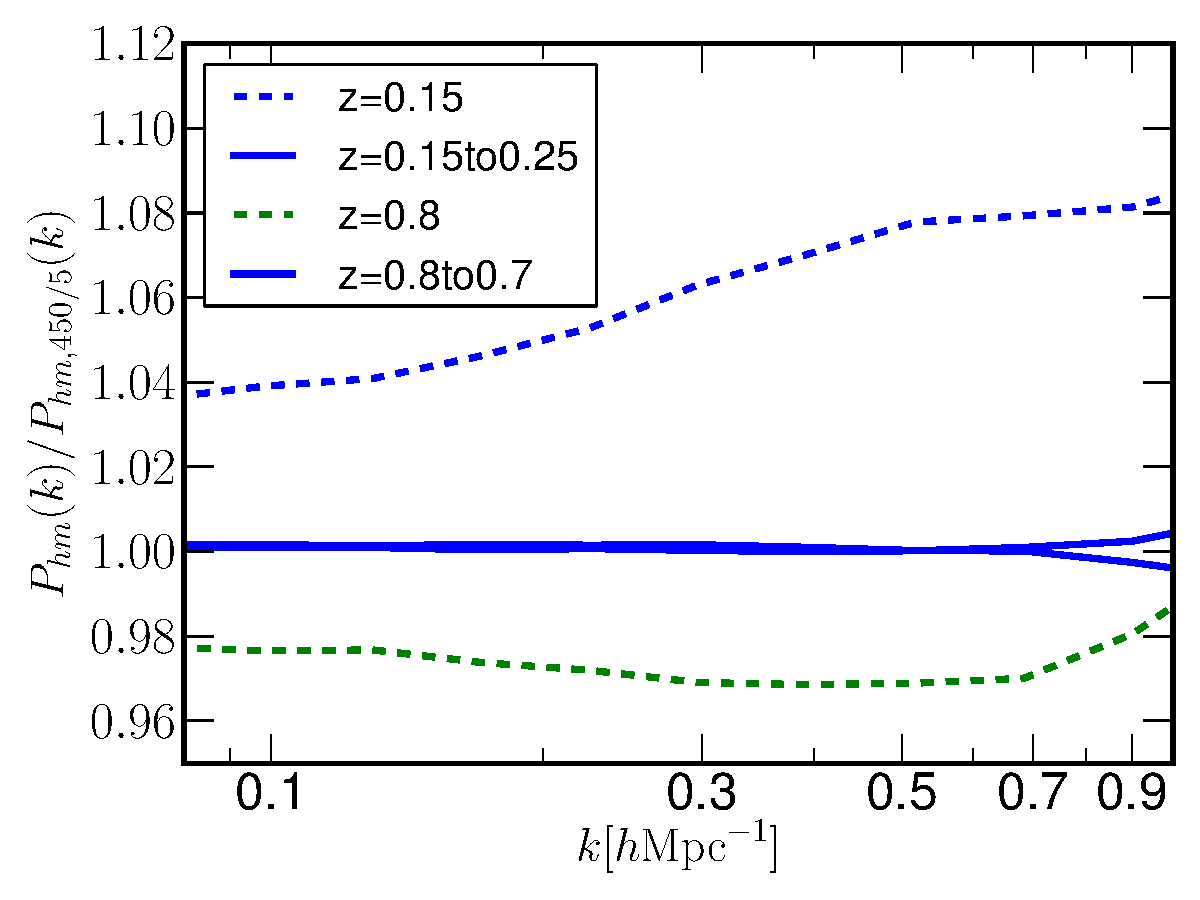
\includegraphics[width=0.5\columnwidth]{\lyxdot \lyxdot /Plots/shifting1}

\caption{\label{fig:power-lightcone}In this figure, we use the halo matter
cross power spectra at $z=0.25$ and $z=0.7$ as a denominator. The
dashed lines show the ratio with the cross power spectra at $z=0.15$
and $z=0.8$ respectively before shifting, and the solid lines are
the ratio after shifting halo positions. It indicates that shifting
the positions of halos from one redshift to the another preserves
the distribution of halos statistically.}
\end{figure}


\begin{figure}[H]
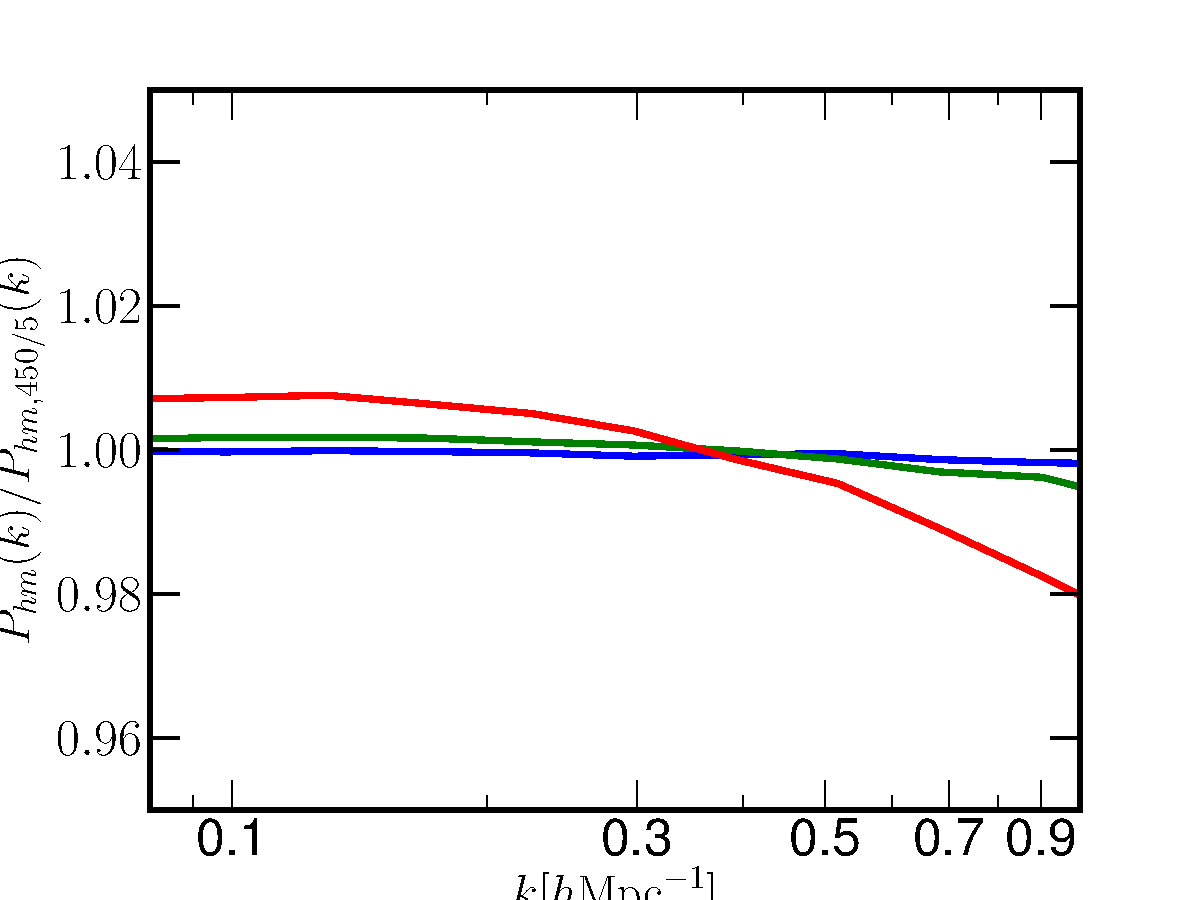
\includegraphics[width=0.5\columnwidth]{\lyxdot \lyxdot /Plots/test1}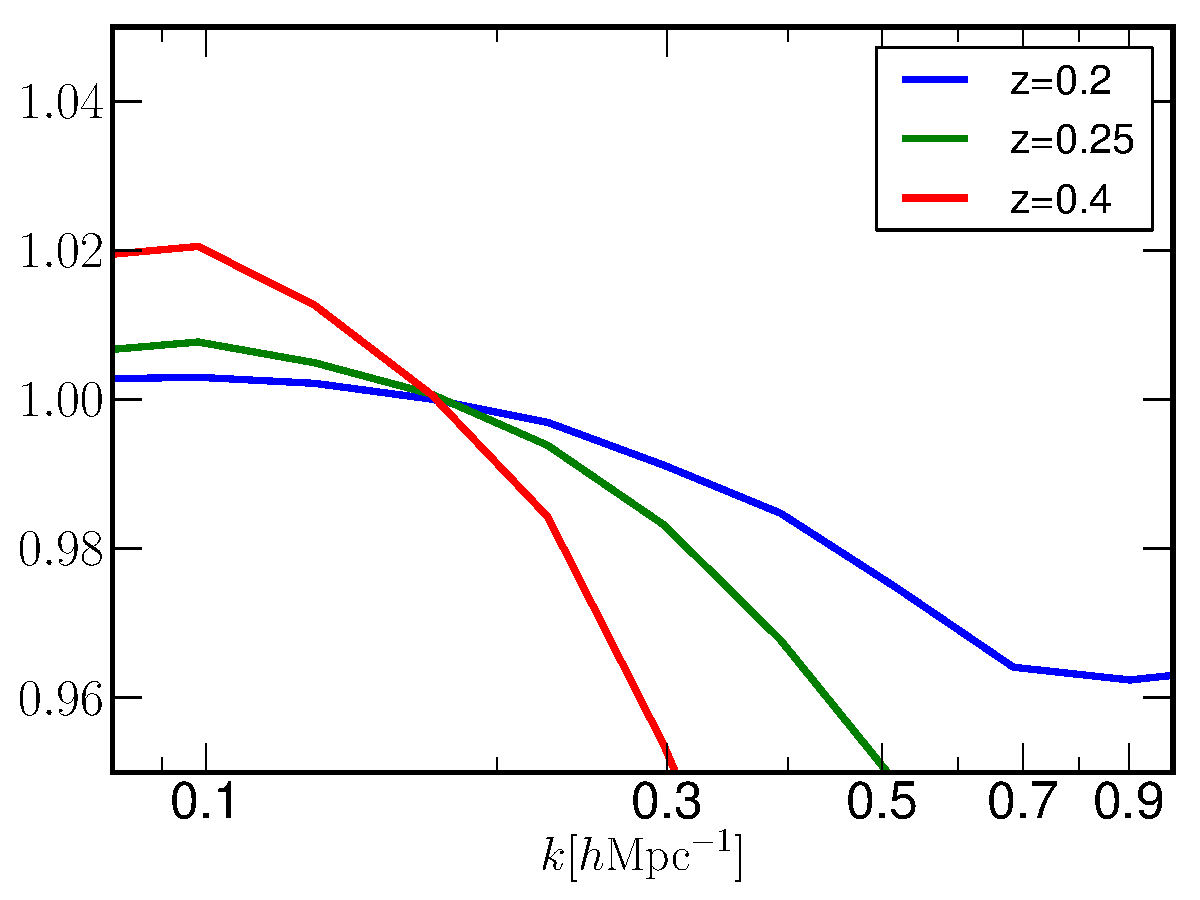
\includegraphics[width=0.5\columnwidth]{\lyxdot \lyxdot /Plots/test2}

\caption{\label{fig:power-lightcone2}Ratio of halo matter cross power spectra
in real space {[}left{]} and in redshift space {[}right{]} after shifting
the position of the halos from the redshift labeled in the plots to
$z=0.15$. The denominator is the cross power spectra at $z=0.15,$where
we use the halo density field in real space and redshift space respectively.
For all cases, we use the DM density field in real space at $z=0.15$. }
\end{figure}


\begin{figure}[H]
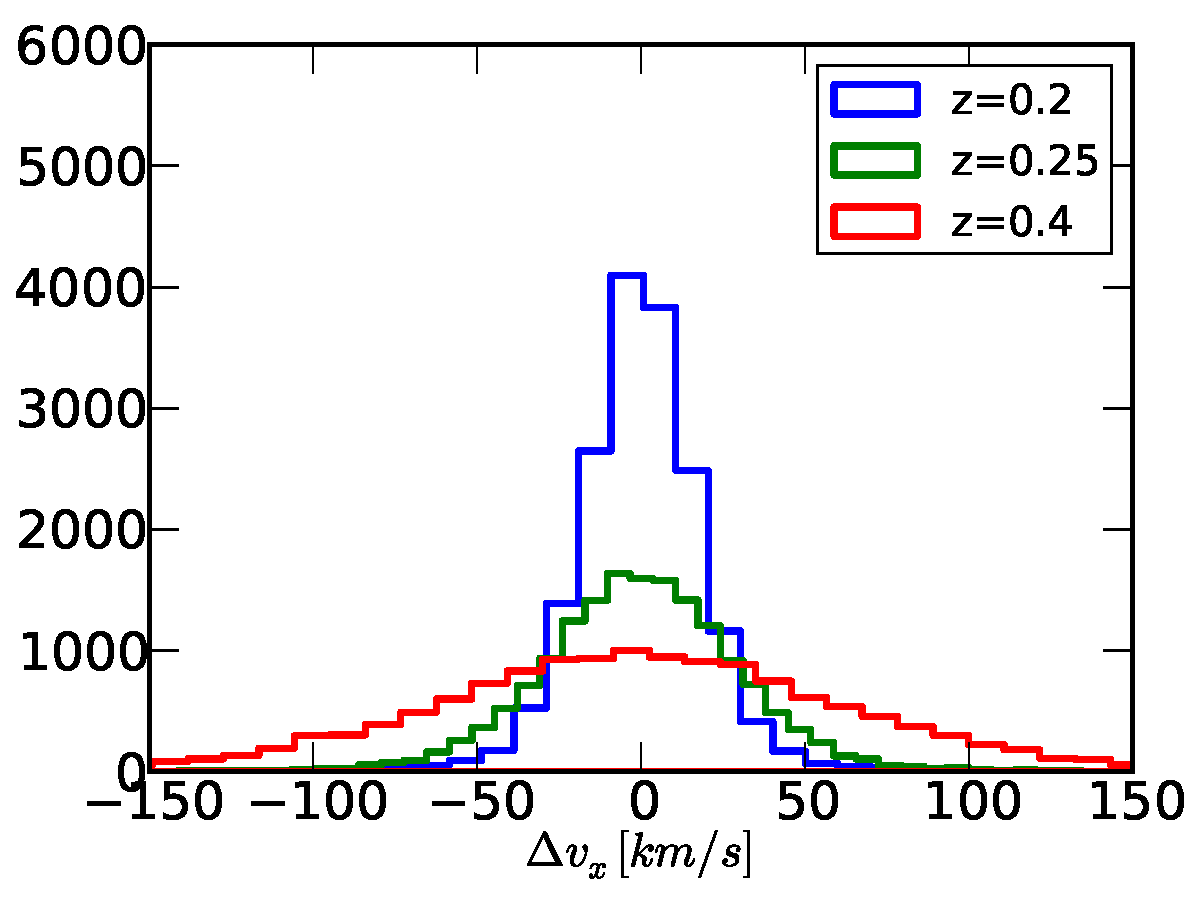
\includegraphics[width=0.5\columnwidth]{\lyxdot \lyxdot /Plots/hist_vx}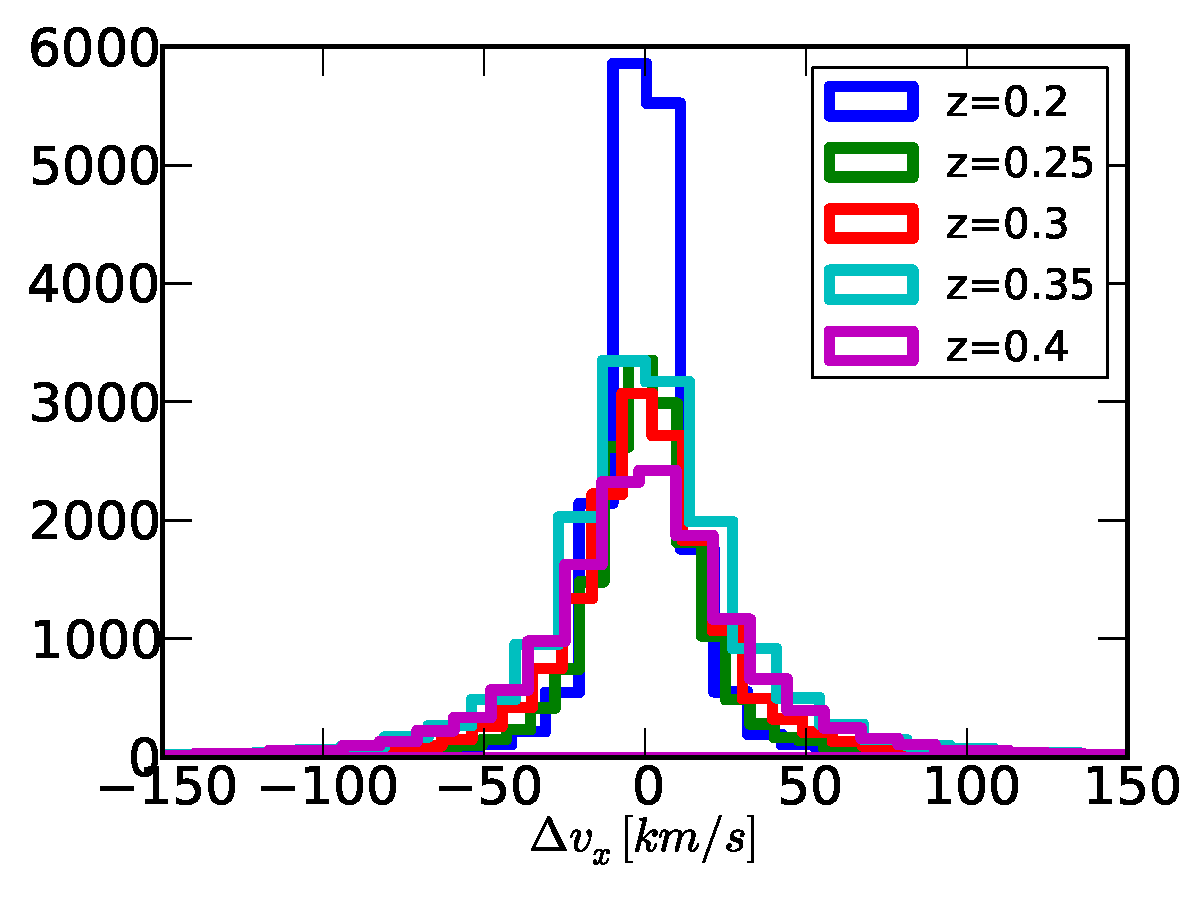
\includegraphics[width=0.5\columnwidth]{\lyxdot \lyxdot /Plots/hist_vx_expFac}

\caption{\label{fig:vel_hist_expFac}Comparisons of the velocities of halos
matched across simulations at different redshifts to the one at $z=0.15$.
From left to right, we compare original halo velocities and the velocities
multiplied by the expansion factor $a(z)$. As shown, the scatter
in the velocity differences decreases in the right panel. This indicates
that the change in velocities at different redshifts is largely affected
by the expansion of the Universe.}
\end{figure}


\begin{figure}
\includegraphics[width=0.5\columnwidth]{\lyxdot \lyxdot /Plots/shifting_s_expFac_z0\lyxdot 15}

\caption{\label{fig:shift-expFac}Ratio of halo matter cross power spectra
in redshift space as shown in Figure \ref{fig:power-lightcone2}.
The only difference is that here we use the velocity field multiplied
by th ratio of the expansion factor $a(z)/a(z=0.15)$ (where z is
the redshift shown in the figure) to compute the halo positions in
redshift-space. The denominator is the cross power spectra at $z=0.15,$where
we use the halo density field in redshift space. For all cases, we
use the DM density field in real space at $z=0.15$.}


\end{figure}



\section{THE BOSS SIMULATIONS}

As a concrete implementation of the approach discussed above, we construct
catalogs designed to mock the Baryon Oscillation Spectroscopic Survey
(BOSS) galaxy samples. BOSS (\cite{2013AJ....145...10D}), part of
the SDSS-III project (\cite{2011AJ....142...72E}), is a spectroscopic
survey that aims to make percent level distance measurements using
the baryon acoustic oscillation technique. The low redshift ($z<0.7$)
distance measurements use two galaxy samples : the LOWZ ($z<0.45$)
and CMASS ($z<0.7$) samples (\cite{2014MNRAS.441...24A,2014MNRAS.440.2222T}).
We focus on the CMASS sample below; however, the same halo catalogs
are useful for the LOWZ sample as well.

We choose a simulation volume large enough to build a full-sky mock
BOSS catalog. Since the CMASS sample extends to $z\sim0.7$, we choose
a simulation side of $4000h^{-1}{\rm Mpc}$,\textcolor{black}{{} corresponding
to a comoving distance to $z\sim0.8$ from the center of the box;
Fig. \ref{fig:boss-geom} shows the BOSS CMASS redshift distribution
as a function of redshift and comoving distance (assuming our fiducial
cosmology). Our simulations are run with $4000^{3}$ particles, corresponding
to a particle mass of $10^{11}{\rm M_{\odot}}$. The characteristic
halo mass for BOSS galaxies corresponds to $10^{13}M_{\odot}$, which
we resolve with 100 particles. We keep all halos down to 40 particles
co}rresponding to a halo mass of $10^{12.6}{\rm M_{\odot}}$. The
simulations are started at \textcolor{red}{$z=200$} with Zel'dovich
initial conditions and are stopped at $z=0.15$ with simulation outputs
every $\Delta z=0.05$. At each of these steps, we store XXX.

The BOSS angular geometry is split into two regions : one in the North
Galactic Cap and one in the South Galactic Cap (Fig. \ref{fig:boss-geom}).
Since we generate full-sky mocks, it is straightforward to embed two
full non-overlapping BOSS surveys in a single mock realization (Fig.
\ref{fig:boss-geom}). We cut out a first BOSS volume with $\vec{x}_{old}$
and then define a new coordinate system $\vec{x}_{new}$ such as $\vec{x}_{new}=R\vec{x}_{old}$,
where $R$ is the Euler rotation matrix for Fig. \ref{fig:boss-geom}:
\[
R=\left(\begin{array}{ccc}
0.088 & 0.096 & 0.991\\
0.219 & -0.973 & 0.075\\
0.972 & 0.211 & -0.107
\end{array}\right).
\]


\begin{figure}
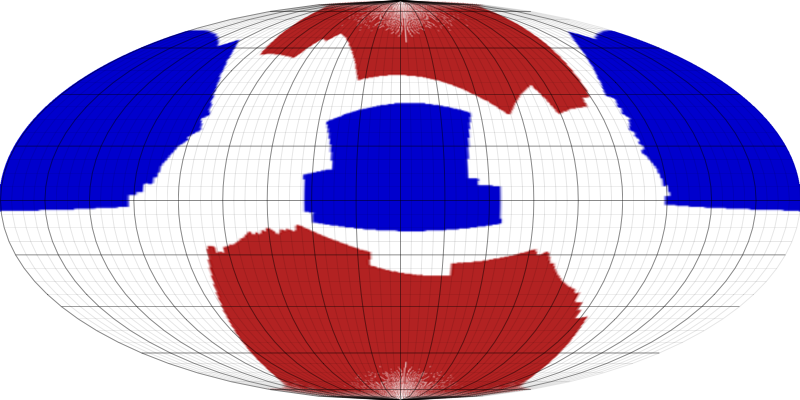
\includegraphics[width=0.5\columnwidth]{\lyxdot \lyxdot /Plots/boss_geom}

\caption{\label{fig:boss-geom}Demonstrating how we fit two non-overlapping
BOSS volumes into the same simulation box. The blue region is the
BOSS survey footprint in equatorial coordinates, while the red region
is the same region rotated using the rotation matrix given in the
text.}
\end{figure}



\subsection{Building the Galaxy Catalog}

To generate galaxy mock catalogs, we need to go through the following
steps:

1) populate halos with galaxies through the HOD functional form,

2) give positions and velocities to the galaxies assuming an NFW profile
\cite{1996ApJ...462..563N}.

The HOD functional form gives probabilities for the number of central
and satellite galaxies based on mass of halos which host those galaxies
with five free parameters. A halo hosts a central galaxy with probability
$N_{cen}(M)$ and a number of satellite galaxies given by a Poisson
distribution with mean $N_{sat}(M)$:

\begin{equation}
N_{cen}(M)=\frac{1}{2}{\rm erfc}\left[\frac{{\rm ln}(M_{cut}/M)}{\sqrt{2}\sigma}\right],\label{eq:Ncen}
\end{equation}
and 
\begin{equation}
N_{sat}(M)=N_{cen}(M)\left(\frac{M-\kappa M_{cut}}{M_{1}}\right)^{\alpha},\label{eq:Nsat}
\end{equation}
where $M_{cut}$, $M_{1}$, $\sigma$, $\kappa$, and $\alpha$ are
free parameters and $M$ is the halo mass. We assume that $N_{sat}(M)$
is zero when $M<\kappa M_{cut}$ and halos do not host satellite galaxies
without a central galaxy (\cite{2005ApJ...633..791Z}). The total
number of galaxies hosted by each halo is a sum of the number of central
and satellite galaxies. Eqs \ref{eq:Ncen} and \ref{eq:Nsat} are
not the only possible functional form for the HOD, and it is trivial
to change this. However, these forms reproduce the clustering of the
BOSS galaxies (\cite{2011ApJ...728..126W}) and we use them in what
follows. 

We place the central galaxies at the center, with a velocity equal
to the halo velocity. We distribute satellite galaxies with an spherically
symmetric NFW profile: 
\begin{equation}
\rho(r)=\frac{4\rho_{s}}{\frac{cr}{R_{vir}}(1+\frac{cr}{R_{vir}})^{2}},
\end{equation}
where $\rho_{s}$ is the density at the char\textcolor{black}{acteristic
scale $r_{s}=R_{vir}/c$ , $R_{vir}$ is the virial radius for the
halo and $c$ determines how centrally concentrated the profile is.
$R_{vir}$ is computed from $M=\frac{4\pi}{3}R_{vir}^{3}\rho_{crit}\Delta_{h}$,
where $\Delta_{h}=(18\pi^{2}+82(\Omega_{m}-1)-39(\Omega_{m}-1)^{2})/\Omega_{m}$
and $\rho_{crit}=\frac{3c^{2}H_{0}^{2}}{8\pi G}$} ($c$ is the speed
of light here). We adopt the form in \cite{2011ApJ...740..102K}:
\begin{equation}
c(M,z)=\frac{c_{0}}{1+z}(M/M_{0})^{-\beta},
\end{equation}
where $c_{0}=9.60$, $M_{0}=10^{12}$, and $\beta=0.075$. There have
been several studies about conecntration, those different expressions
on concentration do not make difference for our purpose.

The velocities of the satellite galaxies are the sum of their host
halo velocity and a random virial component. This random component
are given as follows:

\begin{equation}
<v_{x}^{2}>=<v_{y}^{2}>=<v_{z}^{2}>=\frac{1}{3}\frac{GM}{R_{vir}}.\label{eq:variance}
\end{equation}
We draw a Gaussian distribution with zero mean and variance in Eq.
\ref{eq:variance} to give each component of an internal velocity
for the satellite galaxies. Here, we assume that satellite galaxies
are randomly moving inside the host halos. So, we give the radial
component of this random motion from the Gaussian distribution and
determine the direction randomly with equal probability. 

We generate galaxy mocks from the static snapshots at $z=0.55$. In
Figure \ref{fig:xis}, we compare the correlations function $\xi(s)$
with the one in \textcolor{black}{\cite{2013arXiv1303.4666A}, where
$s$ is the separation in redshift-space. Here, we use the following
HOD parameters, $M_{cut}=12.9$, ,} $\alpha=1.013$,\textcolor{black}{{}
$\kappa=1.0$, $\sigma=0.85$. }

Note that we fit the average number density of galaxies to that of
\cite{2013arXiv1303.4666A} as shown in\textcolor{black}{{} Figure }\ref{fig:nz_gal}.
In order to fit the number density, we randomly select galaxies after
populating halos through HOD.

\textcolor{black}{The correlation function computed from our sample
mocks fits to the correlation function in \cite{2013arXiv1303.4666A}
well on the scale between $30h^{-1}{\rm Mpc}$ and $80h^{-1}{\rm Mpc}$
shown in Figure \ref{fig:xis}. We compute $\chi^{2}$ for monopoles
and quadrupoles from the simulation at $z=0.55$ and the light cone
output. We obtain $\chi^{2}=23.4$ for the simulation at $z=0.55$
and $\chi^{2}=25.0$ for the light cone output. The degree of freedom
here is 14 where $s\in[30h^{-1}{\rm Mpc},78h^{-1}{\rm Mpc}]$. }

\begin{figure}
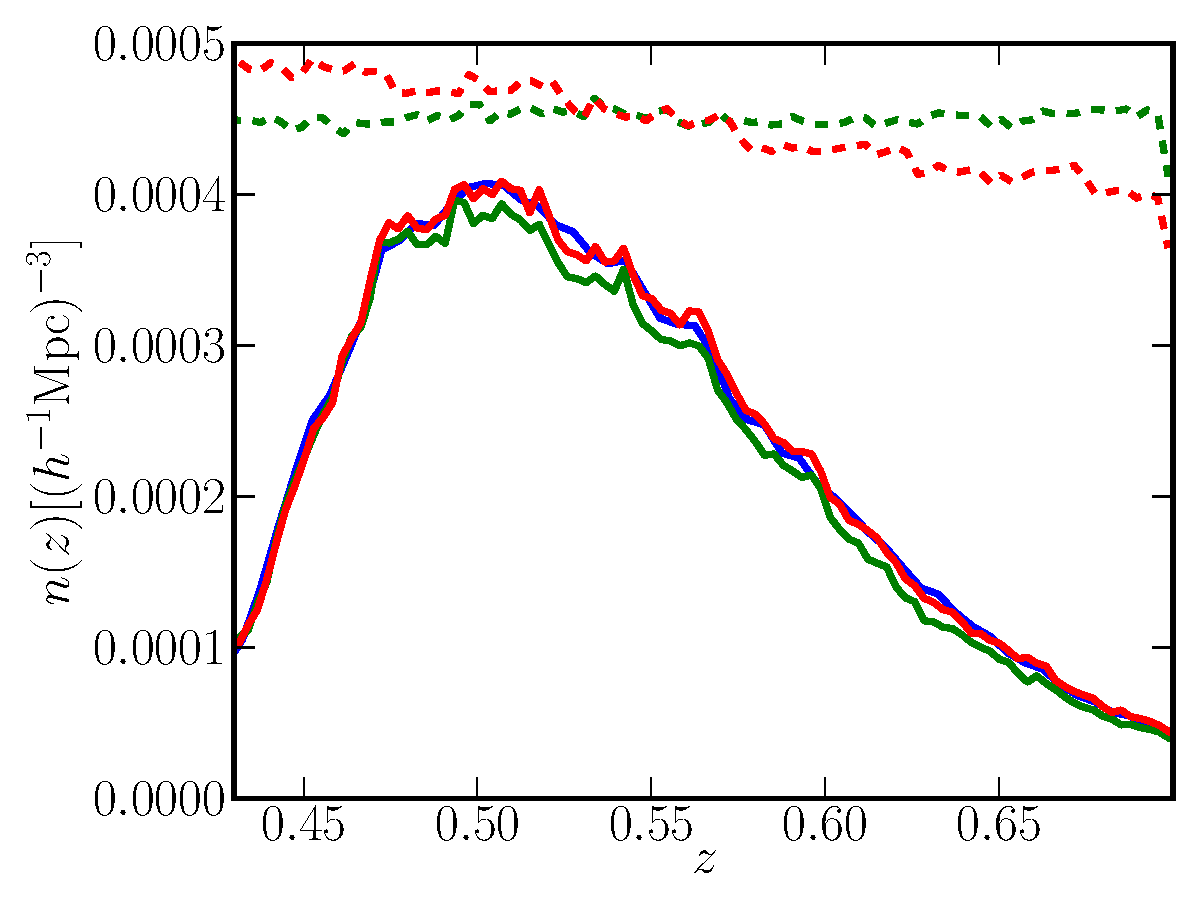
\includegraphics[width=0.5\columnwidth]{\lyxdot \lyxdot /Plots/nz_dr11_N}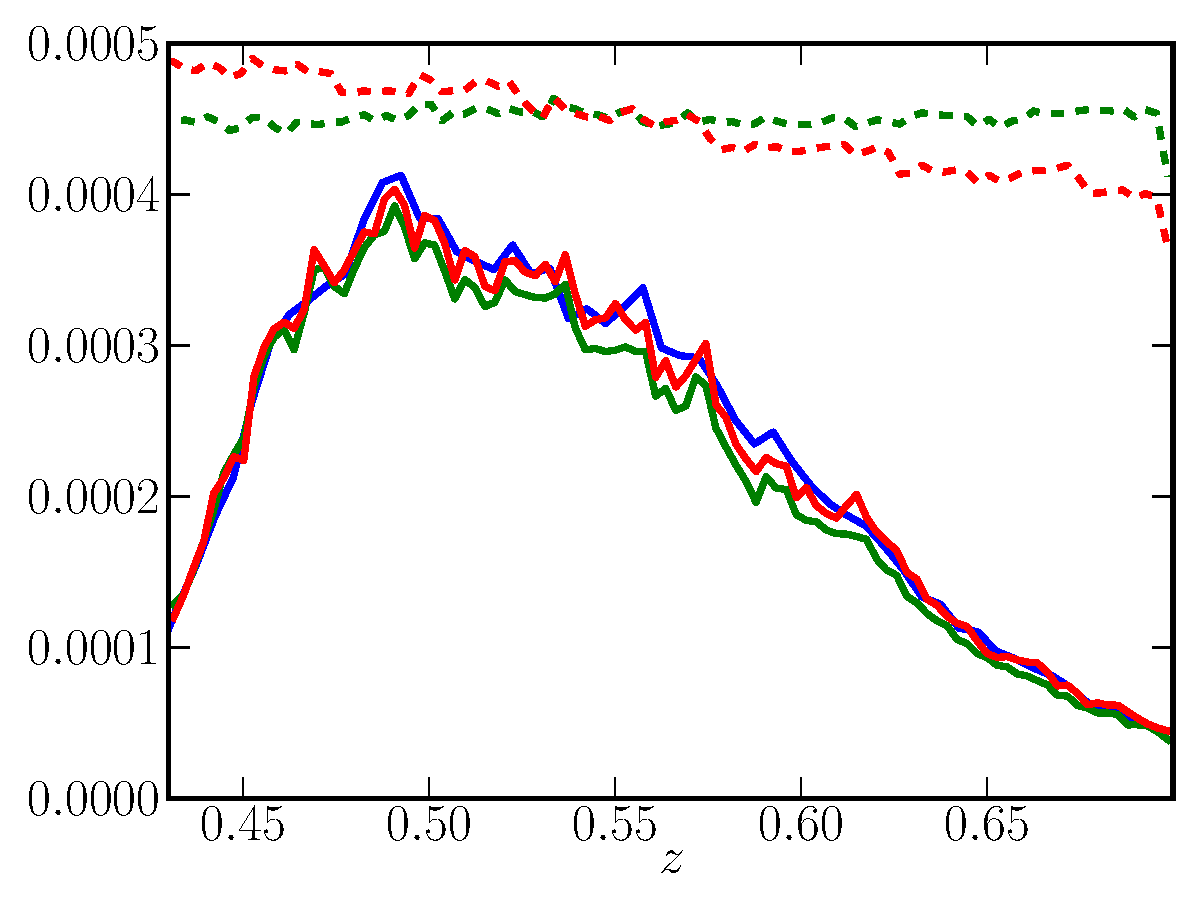
\includegraphics[width=0.5\columnwidth]{\lyxdot \lyxdot /Plots/nz_dr11_S}

\caption{\label{fig:nz_gal}A comparison of galaxy number densities before
fitting to DR11 {[}dashed lines{]} and after {[}solid lines{]}. The
blue solid line is $n(z)$ from DR11 (North) in \cite{2013arXiv1303.4666A}.
The green and red lines are from the mocks at $z=0.55$ and the lightcone
output respectively. The HOD parameters used to generate the mock
catalogs can be found in text.}
\end{figure}


\begin{figure}
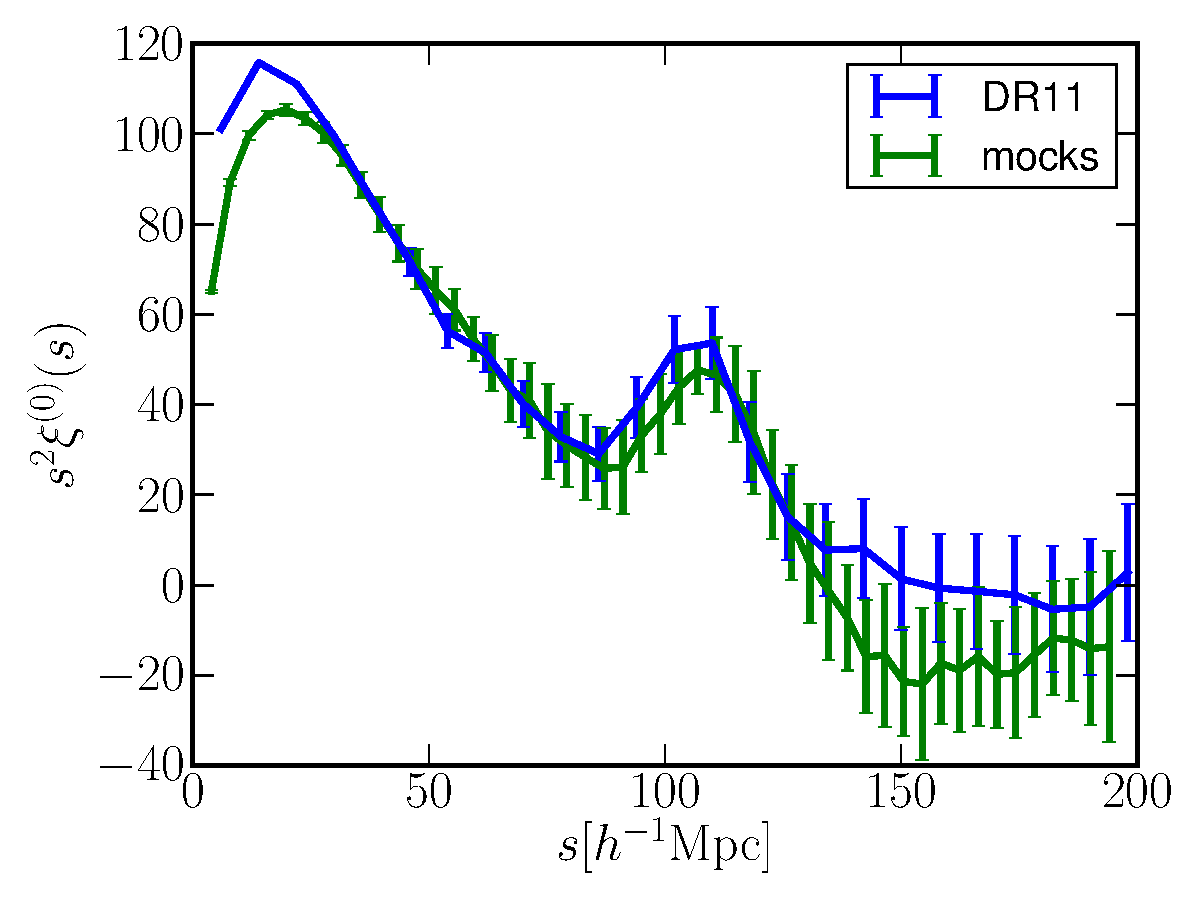
\includegraphics[width=0.5\columnwidth]{\lyxdot \lyxdot /Plots/xi0_obs}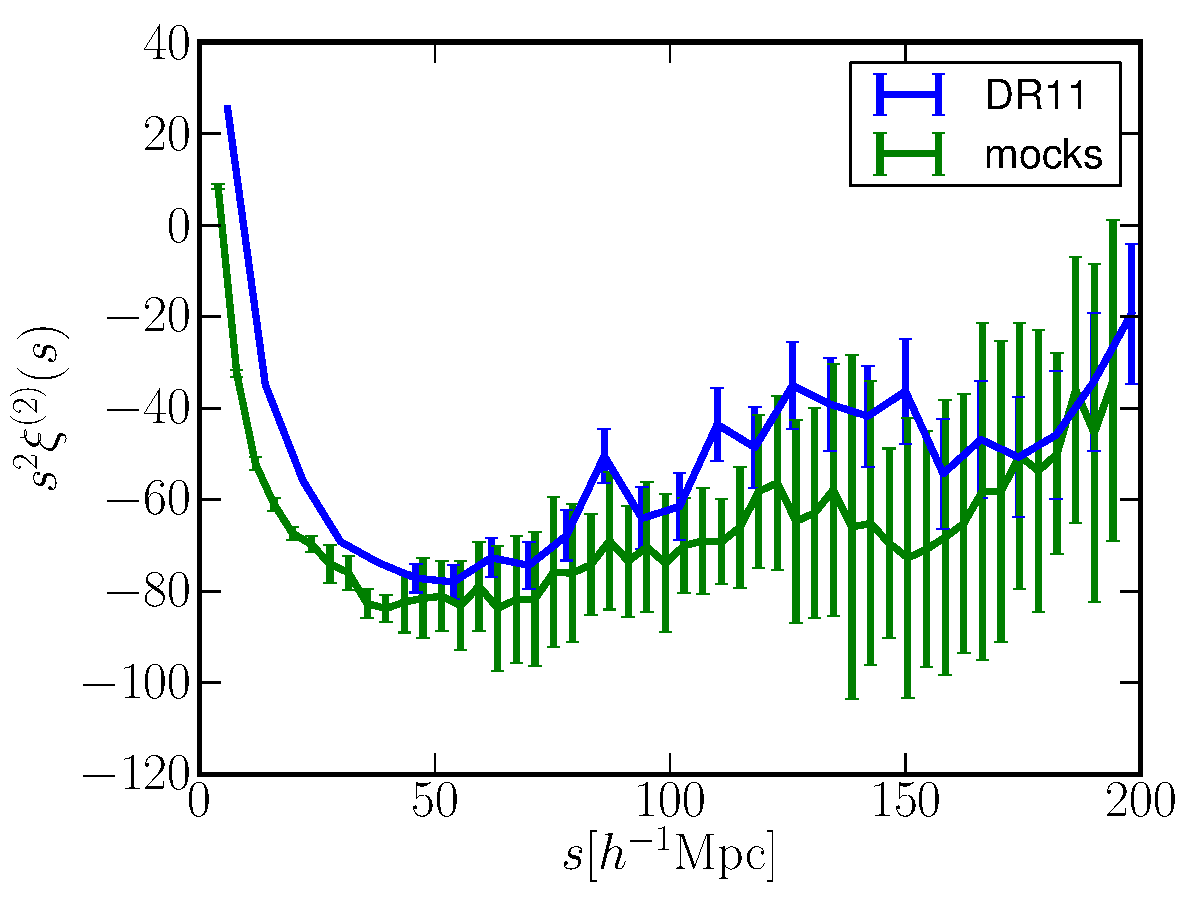
\includegraphics[width=0.5\columnwidth]{\lyxdot \lyxdot /Plots/xi2_obs}

\caption{\label{fig:xis}Correlation function monopoles $\xi^{(0)}(s)$ {[}left{]}
and quadrupoles $\xi^{(2)}(s)$ {[}right{]} of the mocks (green) and
DR11 in \textcolor{red}{\citet{2013arXiv1303.4666A}} (blue) at $z=0.55$.
The HOD parameters used to generate the mock catalogs can be found
in text. }
\end{figure}



\section{Discussion}

Precision required for current and future galaxy spectroscopic surveys
to test the expansion and structure formation histories of the Universe
requires an accurate understanding of systematic effects. In this
paper we have presented a quantitative study of the impact of time
step sizes on the halo and matter density fields. Our code has two
adjustable time stepping parameters - a global time step and a number
of sub-cycles (responsible for a particle-particle interactions) to
track that particle trajectories on small scales. We consider cases
where we increase the length of each time step by factors of 1.5 and
3 respectively, as well as reducing the number of sub-cycles. Our
fiducial choice is to use using 300 global time steps corresponding
to $\Delta a(z)=0.003$ and 2 sub-cycles (increasing the length of
the global time step by a factor of 1.5 and that of the sub-cycles
by a factor of 2.5), resulting in a reduction of the simulation run
time by 4 times less. We keep the mass resolution constant; the results
here are based on a particle mass of $5.3\times10^{10}h{\rm M_{\odot}}$.We
summarize the key results below: 

(a) The halo masses tend to be underestimated in these cases, as one
might expect because reducing the number of time steps produces halos
with less substructure and a more diffuse distribution of mass. However,
this trend may be calibrated with smaller simulations and corrected,
recovering the halo masses to 98\%. The halo mass function is correctly
recovered fully for masses above $10^{12.7}h^{-1}{\rm M_{\odot}}$
corresponding to 100 particles. Note that we run the halo finder with
identical parameters as in the full resolution runs. It may however
be possible to get similar results by changing the parameters of the
halo finder, as was done in \cite{2013MNRAS.428.1036M}.

(b) \textcolor{black}{The halo positions and velocities are recovered
with a scatter of $0.08[h^{-1}{\rm Mpc}]$ and $12.8[{\rm km/s}]$
respectively for the simulation of our fiducial choice. }

(c) The clustering of these halos is correctly recovered to better
than 1\% on scales below $k<1[h{\rm Mpc^{-1}]}$ in real-space and
$k<0.5[h{\rm Mpc^{-1}}]$.

(d) We find that the number of sub-cycles makes almost no difference
to any of our final results.

\textcolor{black}{We also consider the redshift sampling required
to construct light cone outputs. We first compare the distances for
the halos at different redshifts before and after shifting their positions
from one redshift to the another. Moving halos over a $\Delta z=0.1$
interval correctly reduecs the standard deviation of those distances
from $0.25[h^{-1}{\rm Mpc}]$ to}\textcolor{red}{{} }\textcolor{black}{$0.09[h^{-1}{\rm Mpc}]$.
Moreover, the power spectra are correctly recovered to better than
1\% for $k<0.5[h{\rm Mpc^{-1}]}$ for $\Delta z=0.25$. This worsens
in redshift space to 2\% up to $k<0.2[h{\rm Mpc^{-1}]}$.}\textcolor{red}{{}
}\textcolor{black}{The agreement is, however, improved to 1\% for
$k<1[h{\rm Mpc^{-1}]}$ by using the velocity scaled by the relative
scale factor between the snapshot and the true redshift. Our fiducial
choice to construct light cone outputs is $\Delta z=0.05$.}

This work is a natural extension of the approaches described in \cite{2014MNRAS.439L..21K,2014MNRAS.437.2594W,2014arXiv1409.1124C,2013MNRAS.428.1036M,2014arXiv1401.4171M}.
The primary goal for those papers was to generate the large numbers
of simulations required for estimating covariance matrices. We quantify,
in detail, the impact of size of the time step on large scale observables;
our suite of simulations are better designed for testing for systematic
errors in theory and analysis techniques. As a proof of principle,
we present a set of eight full BOSS (both North and South Galactic
caps simultaneously) simulations. The time savings presented in this
paper allowed to extend this to 50 simulations, across a range of
cosmologies. These results from these will be presented in future
publications.


\section*{Acknowledgement}

\bibliographystyle{plainnat}
\bibliography{bigsims}

\end{document}
